\documentclass{article}
\usepackage{amsrefs}
\usepackage{amssymb}
\usepackage{enumerate}
\usepackage{amsmath}
\usepackage{amsthm}
\usepackage{graphicx}
\usepackage{amssymb,latexsym}
\usepackage{graphicx}
\DeclareMathOperator{\dom}{dom}

\begin{document}

\begin{itemize}
\item Wat is een differentiaal?
\item Hoe geeft de kettingregel voor het afleiden de methode van substitutie voor het onbepaald integreren?
\item Hoe gebruik je de methode van substitutie voor het onbepaald integreren?
\end{itemize}

\vspace{2mm}

Voor een functie $y=f(x)$ en $a \in \dom f$ is $Df(a)$ de richtingsco\"effici\"ent van de raaklijn $T$ aan de grafiek $G$ van $f$ in $P(a,f(a))$.
De vergelijking van de raaklijn is dan
\[
y-f(a)=Df(a).(x-a) \text { .}
\]
Het punt op die raaklijn dat behoort bij $x=a$ voldoet aan $y=f(a)$ en is dus $P(a;f(a))$ (wat logisch is).
Als je bij die $x$-waarden $\Delta x$ bijtelt dan vul je $x=a+\Delta x$ in.
Je bekomt dan de volgende waarde van $y$ op de raaklijn:
\[
y-f(a)=Df(a).(a+\Delta x -a)=Df(a).\Delta x
\]
\[
y=f(a)+Df(a).\Delta x \text { .}
\]
De verandering van de $y$-waarde op de raaklijn is dan
\[
\Delta y=Df(a).\Delta x \text { .}
\]
\begin{figure}[h]
\begin{center}
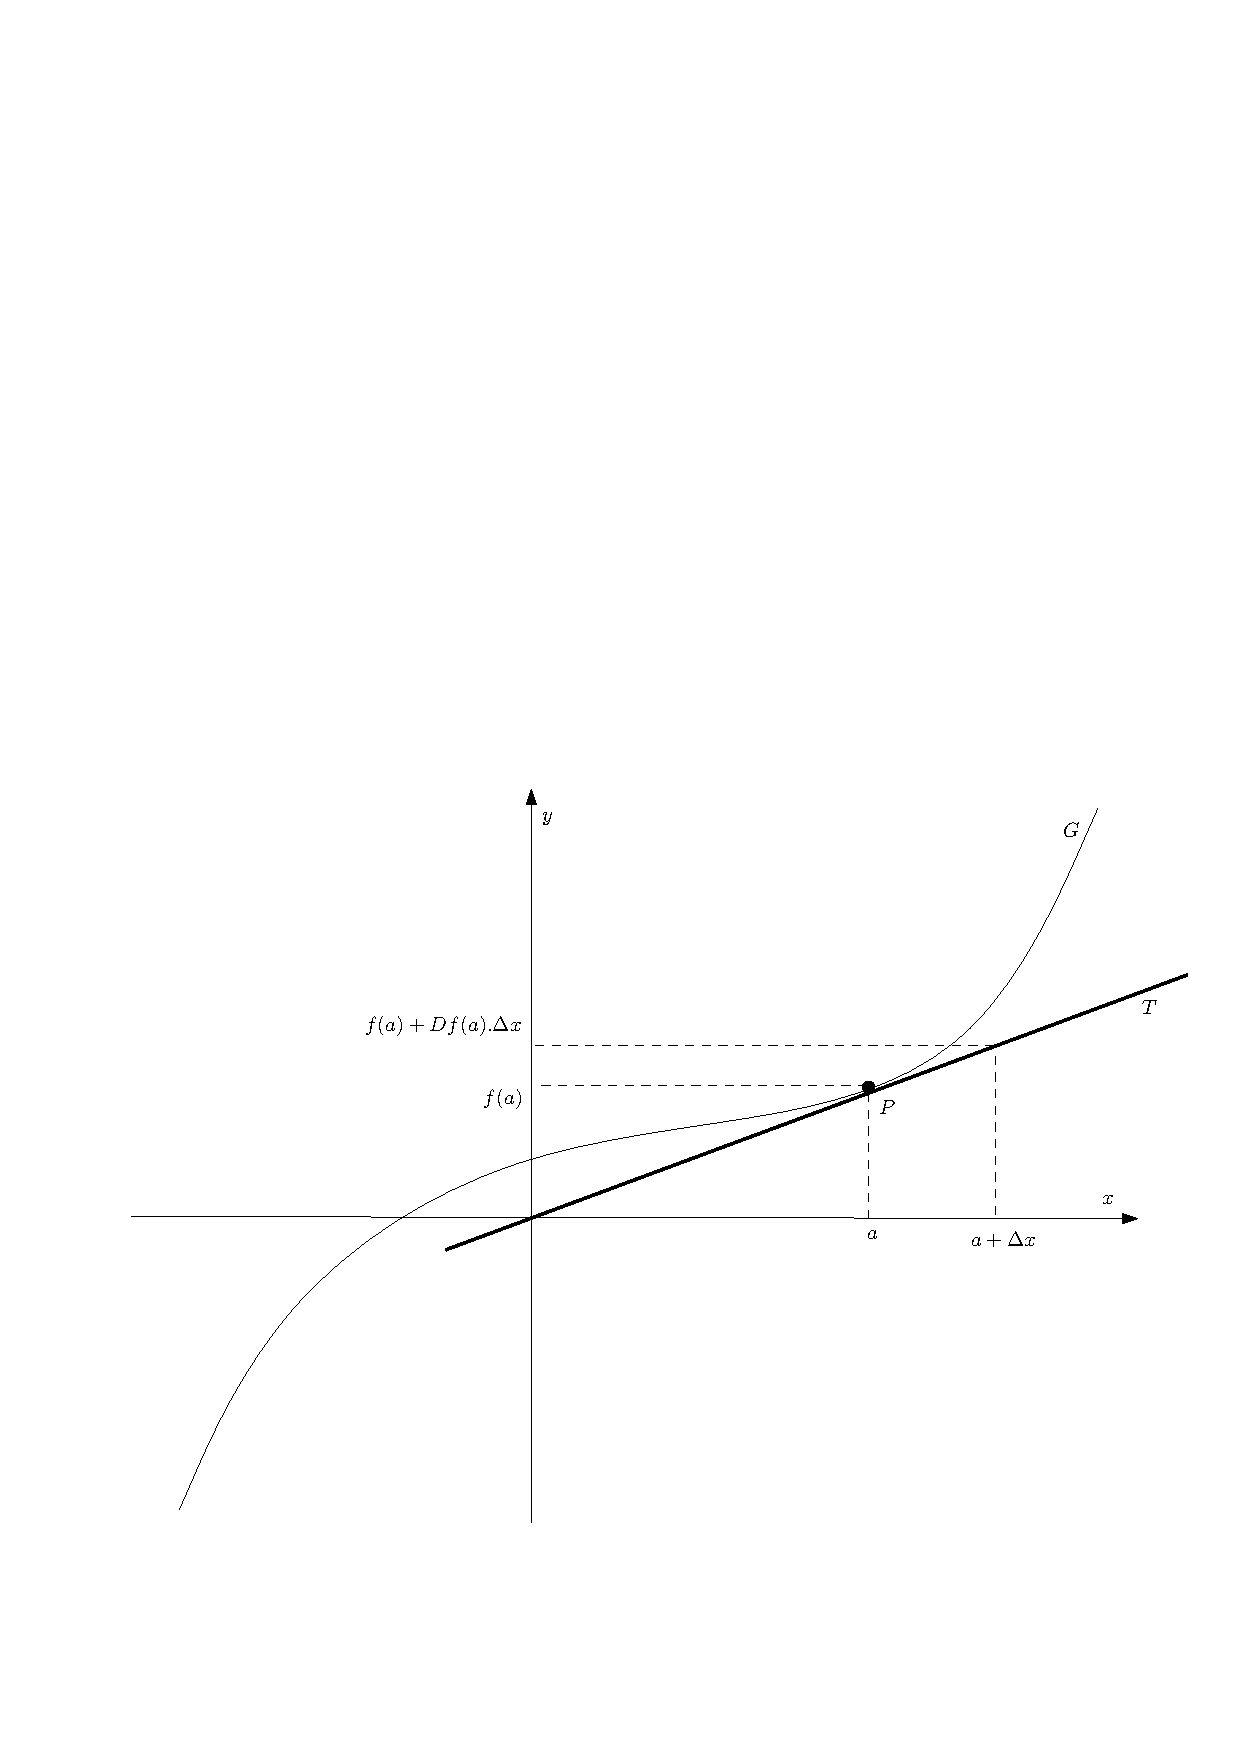
\includegraphics[height=5 cm]{substitutie1.pdf}
\end{center}
\end{figure}
Hierdoor wordt $\Delta y$ een functie in $\Delta x$ en je noemt deze functie de differentiaal van $f$ in $a$.
Je noteert  $df(a)$ voor deze functie, dus
\[
df(a)=Df(a).\Delta x \text { .}
\]
Neem je als bijzonder geval $f(x)=x$ dan is $Df(a)=1$ en dus $df(a)=\Delta x$.
Deze functie in $\Delta x$ noem je de differentiaal van $x$ en je schrijft $dx$.
Je bekomt dus
\[
dx=\Delta x \text { .}
\]
Daarom schrijft men ook
\[
df(a)=Df(a).dx \text { .}
\]
Let wel op: het gaat hier over twee functies in de veranderlijke $\Delta x$ die een veelvoud zijn van elkaar.

Als je de oorspronkelijke functie noteert als $y=f(x)$ dan schrijf je ook $dy(a)$ in plaats van $df(a)$.
Je bekomt dan
\[
dy(a)=Df(a).dx \text { .}
\]
Vervang je $a$ door een willekeurig getal $x$ dan schrijf je
\[
dy=Df(x).dx \text { .}
\]
Een onbepaalde integraal van een functie $y=f(x)$ genoteerd $\int f(x)dx$ kun je ook opvatten als een onbepaalde integraal van de differentiaal $f(x)dx$.\\

Uit de kettingregel voor het afleiden vinden we
\[
\int Dg(f(x))Df(x)=g(f(x))+C \text { .}
\]
Stel nu $u=f(x)$, dan is $du=Df(x)dx$ en dan bekom je
\[
\int Dg(f(x))Df(x)=\int Dg(u)du \text { .}
\]
Per definitie is $\int Dg(u)du=g(u)+C$ en door $u$ terug in te vullen vind je
\[
\int Dg(f(x))Df(x)dx=\int Dg(u)du=g(u)+C=g(f(x))+C \text { .}
\]
Omdat je in deze redenering $f(x)$ vervangt (substitutie) door een variabele $u$ noem je dit de methode van substitutie.
Het is gewoon een handige werkwijze om de kettingregel van het afleiden te gebruiken voor het berekenen van een onbepaalde integraal.\\

We hermaken nu de twee laatste voorbeelden uit vorig deel.\\

\noindent $\int \sqrt[3]{x+7} dx$

Stel $u=x+7$, dan is $du=D(x+7)dx=dx$.
Je bekomt
\[
\int \sqrt[3]{x+7}dx=\int \sqrt[3]{u}du=\int u^{1/3} du=
\]
\[
=\frac{u^{4/3}}{4/3}+C=\frac{3u^{4/3}}{4}+C=\frac {3\sqrt[3]{(x+7)^4}}{4}+C \text { .}
\]

\vspace{2mm}

\noindent $\int \sin (2x-5)dx$.

Stel $u=2x-5$ dan is $du=D(2x-5)dx=2dx$, dus $dx=\frac{du}{2}$.
Je hebt
\[
\int \sin (2x-5)dx=\int \sin(u) \frac{du}{2}=\frac{1}{2} \int \sin (u)du=
\]
\[
=-\frac{1}{2} \cos (u)+C=\frac{1}{2} \cos (2x-5)+C \text { .}
\]

\vspace{2mm}

Een iets moeilijker voorbeeld dat aantoont dat je niet steeds $dx$ moet vervangen: $\int \frac{xdx}{x^2+1}$.
\noindent (Dit lijkt mij geschikt om door middel van een filmpje te geven.)

Stel $u=x^2+1$ dan is $du=2xdx$ en dus $xdx=\frac{du}{2}$.
Je bekomt
\[
\int \frac{xdx}{x^2+1}=\int \frac{du/2}{u}=\frac{1}{2} \int \frac{du}{u}=
\]
\[
=\frac{1}{2} \ln \vert u \vert +C=\frac{1}{2} \ln \left( x^2+1 \right)+C=\ln \left( \sqrt{x^2+1} \right)+C \text { .}
\]







\end{document}